\documentclass[aspectratio=169]{beamer}

\usepackage{calc}
\usepackage{graphicx}
\usepackage{siunitx}
\usepackage{xcolor}

\graphicspath{{./images}}
\setbeamertemplate{navigation symbols}{}

\author{Chris Doble}
\date{}
\subtitle{Building a GPS receiver from scratch}
\title{Part 5: Acquisition}
\usetheme{Madrid}

% Show the topics frame at the start of each section
\AtBeginSection[]
{
  \begin{frame}
    \frametitle{Topics}
    \tableofcontents[currentsection, subsubsectionstyle=hide]
  \end{frame}
}

% Show the topics frame at the start of each subsection
\AtBeginSubsection[]
{
  \begin{frame}
    \frametitle{Topics}
    \tableofcontents[currentsection, currentsubsection, subsubsectionstyle=hide]
  \end{frame}
}

% Show the topics frame at the start of each subsubsection
\AtBeginSubsubsection[]
{
    \begin{frame}
        \frametitle{Topics}
        \tableofcontents[currentsection, currentsubsection, subsubsectionstyle=show/shaded]
    \end{frame}
}

\begin{document}

\frame{\titlepage}

\begin{frame}
    \frametitle{Topics}

    \tableofcontents[subsubsectionstyle=hide]
\end{frame}

\section{Parameters}

\subsection{PRN code phase}

\begin{frame}
    \frametitle{PRN code phase}

    \begin{itemize}
        \item To decode satellite $i$'s navigation message bit, calculate \[\int_{t_0}^{t_0 + 0.001} r(t) \hat{PRN}_i(t) \,d t\] where $t_0$ is a point in time and $r(t)$ is the received signal
        
        \begin{itemize}
            \item<2-> PRN codes aligned $\Rightarrow$ navigation message bit
            
            \item<3-> PRN codes misaligned $\Rightarrow$ noise
        \end{itemize}

        \item<4-> In order to align them, we need to know the phase
    \end{itemize}
\end{frame}

\subsection{Carrier wave frequency shift}

\begin{frame}
    \frametitle{Topics}

    \tableofcontents[currentsection, currentsubsection, subsubsectionstyle=show]
\end{frame}

\subsubsection{Modulation signal, misaligned PRN code}
\subsubsection{Modulation signal, aligned PRN code}
\subsubsection{Modulated signal, not frequency shifted}

\begin{frame}
    \frametitle{Modulated signal, not frequency shifted}

    \begin{itemize}
        \item $\hat{D}_i(t) \hat{PRN}_i(t) f(t)$
        
        \item<2-> Bandpass sampling results in $f(t) \Rightarrow A e^{j \phi}$
        
        \item<3-> Samples will be equal to $\pm A e^{j \phi}$
    \end{itemize}
\end{frame}

\subsubsection{Modulated signal, frequency shifted}

\begin{frame}
    \frametitle{Modulated signal, frequency shifted}

    \begin{itemize}
        \item $\hat{D}_i(t) \hat{PRN}_i(t) g(t)$
        
        \item<2-> A frequency shifted signal $\Leftrightarrow$ a signal with a constantly changing phase
        
        \item<3-> Bandpass sampling results in $g(t) \Rightarrow A e^{j (2 \pi \Delta f t + \phi)} = A e^{j \phi} e^{j 2 \pi \Delta f t}$
        
        \item<4-> Samples will be equal to $\pm A e^{j \phi} e^{j 2 \pi \Delta f t}$
    \end{itemize}
\end{frame}

\begin{frame}
    \frametitle{Recovering the signal}

    \begin{itemize}
        \item<2-> Undo the rotation by multiplying each sample by $e^{-j 2 \pi \Delta f t}$
        
        \item<3-> This is called carrier wipeoff and it's why we need to know $\Delta f$
    \end{itemize}
\end{frame}

\section{Finding parameters}

\begin{frame}
    \frametitle{Finding parameters}

    \centering
    \only<1>{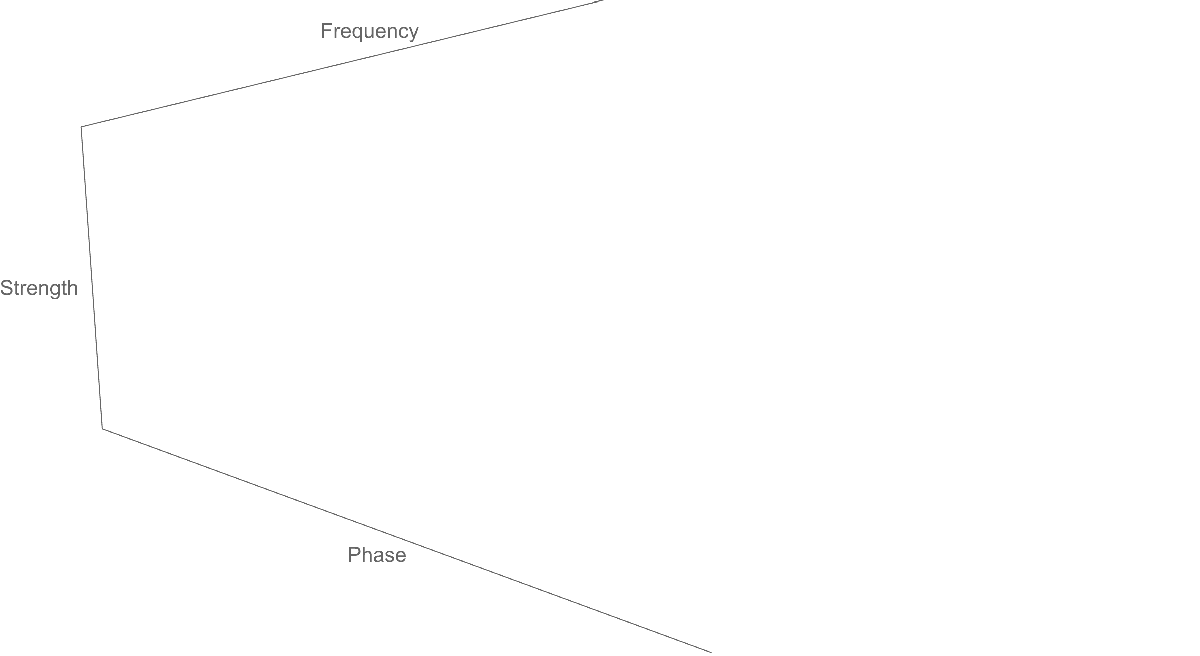
\includegraphics[width=\textwidth * 3 / 4]{1 acquisition space axes.pdf}}%
    \only<2>{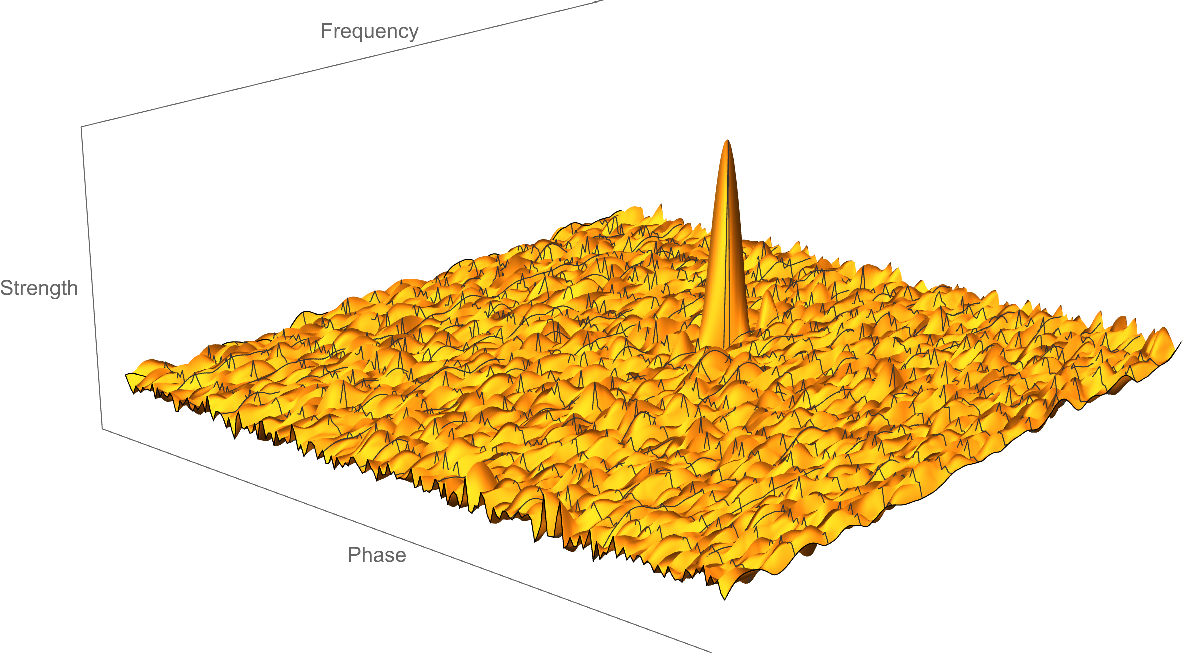
\includegraphics[width=\textwidth * 3 / 4]{2 acquisition space.pdf}}
\end{frame}

\begin{frame}
    \frametitle{Finding parameters}

    \begin{itemize}
        \item<2-> We want to calculate the correlation over a $\qty{10}{ms}$ period
        
        \item<3-> There's a higher chance that the navigation message bit will change
        
        \item<4-> If it does, some samples will cancel each other out $\Rightarrow$ smaller correlation
        
        \item<5-> Calculate correlation over $10 \times \qty{1}{ms}$ periods, add their magnitudes
        
        \item<6-> This is called non-coherent integration
    \end{itemize}
\end{frame}

\section{Parameter space}

\begin{frame}
    \frametitle{PRN code phase}

    \begin{itemize}
        \item $f_s = \qty{2.046}{MHz} \Rightarrow \qty{2046}{samples/ms}$
        
        \item<2-> PRN code is 1023 bits long, repeats once per $\unit{ms}$
        
        \item<3-> Upsample the PRN code to be 2046 half-bits long
        
        \item<4-> There are 2046 phases to check
    \end{itemize}
\end{frame}

\begin{frame}
    \frametitle{Carrier frequency shift}

    \begin{itemize}
        \item<2-> $\Delta f$ due to satellite motion $\pm \qty{4.9}{kHz}$
        
        \item<3-> $\Delta f$ due to Earth's rotation $\pm \qty{2.4}{kHz}$
        
        \item<4-> $\Delta f$ due to receiver motion $\pm \qty{150}{Hz}$
        
        \item<5-> $\Delta t_\text{total} \approx \pm \qty{7.5}{kHz}$
    \end{itemize}
\end{frame}

\section{Determining presence}

\begin{frame}
    \frametitle{Determining presence}

    \begin{enumerate}
        \item On startup, find the best parameters and signal strength for every satellite
        
        \item<2-> Compare the signal strength with a threshold
        
        \item<3-> If it's greater $\Rightarrow$ present
        
        \item<4-> If it's smaller $\Rightarrow$ absent

        \item<5-> Periodically try to acquire satellites we're not tracking
    \end{enumerate}
\end{frame}

\begin{frame}
    \frametitle{Recap}

    \begin{itemize}
        \item<2-> Two required parameters
        
        \begin{itemize}
            \item<3-> PRN code phase $\Rightarrow$ align the PRN codes
            
            \item<4-> Carrier frequency shift $\Rightarrow$ undo the effects of frequency shift (carrier wipeoff)
        \end{itemize}

        \item<5-> These parameters are found by brute force
        
        \item<6-> Size of the parameter space
        
        \begin{itemize}
            \item<7-> PRN code phase $\Rightarrow [0, 2046)$
            
            \item<8-> Carrier frequency shift $\Rightarrow \pm \qty{7.5}{kHz}$
        \end{itemize}

        \item<9-> Determining presence

        \begin{enumerate}
            \item<10-> Calculate the best parameters and signal strength
            
            \item<11-> Compare the signal strength against a threshold
            
            \item<12-> If above the threshold $\Rightarrow$ present
            
            \item<13-> If below the threshold $\Rightarrow$ absent, check again later
        \end{enumerate}
    \end{itemize}
\end{frame}

\end{document}